\documentclass{article}

\usepackage[italian]{babel}
\usepackage[utf8]{inputenc}
\usepackage{hyperref}
\usepackage{natbib}
\usepackage{graphicx}
\usepackage{float}
\usepackage[margin=2.5cm]{geometry}
\usepackage{wrapfig}
\usepackage{minted}

\title{ATTSW Exam}
\author{Gabriele Puliti - \texttt{5300140} - \href{mailto:gabriele.puliti@stud.unifi.it}{\textit{gabriele.puliti@stud.unifi.it}}}
\date{December 2017}

\begin{document}

\maketitle

\begin{flushleft}

% https://docs.gradle.org/current/userguide/userguide.html

\section{Gradle} % https://github.com/gradle/gradle 
Gradle è un progetto open source che fornisce un tool di build automation, che può essere un ottimo sostituto di Maven. Offre un modello in grado di sostenere l'intero ciclo di vita dello sviluppo del software ed è stato progettato per supportare build automation attraverso più linguaggi e piattaforme. Nel nostro caso considereremo questo tool per lo sviluppo di software Java.


\subsection{Differenze tra Gradle e Maven} % https://gradle.org/maven-vs-gradle/
Ci sono molte differenze tra questi due tools: flessibilità, performance, gestione delle dipendenze e molto altro. La configurazione di Gradle in un progetto ha una convenzione molto più facile e comprensibile rispetto alla tediosa e a volte impossibile configurazione del pom.xml di Maven, anche se entrambi usano dei metodi di miglioramento della velocità di esecuzione delle build. Grandle usufruisce di:
\begin{itemize}
    \item \textbf{Incrementality:} evitando il lavoro di monitoraggio dei task di I/O eseguendo solo il necessario e quando possibile processare solo i files che sono cambiati;
    \item \textbf{Build Cache:} utilizza un sistema di cache riusando gli outputs di altre build Gradle con gli stessi inputs;
    \item \textbf{Deamon:} sfrutta un long-lived process che mantiene tutte le informazioni in memoria.
\end{itemize}
Queste 3 caratteristiche rendono Gradle molto veloce, ad esempio una build Gradle con Maven verrebbe completata con un tempo 3 volte maggiore. Tutto questo è anche possibile grazie a un sistema di esecuzioni parallele di task e intra-task.
\begin{figure}[H]
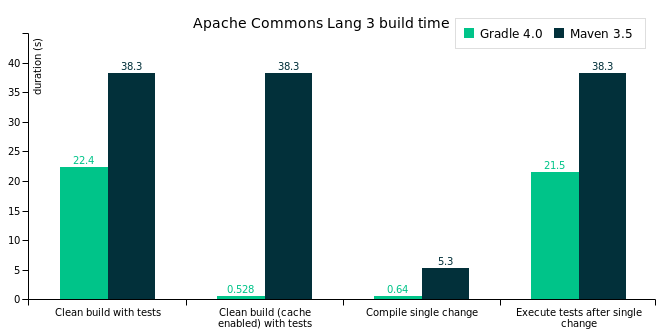
\includegraphics[scale=0.70]{performance.png}
\end{figure} 
% https://docs.gradle.org/current/userguide/userguide.html

\subsection{Installazione}
L'istallazione di Gradle può essere fatta in più modi: tramite installazione manuale o utilizzando un package manager (tutte le informazioni possono essere trovate in \textbf{\href{https://gradle.org/install/}{questo link}}). Personalmente consiglio l'utilizzo del software development kit manager \textbf{\href{http://sdkman.io/}{SDKMAN!}} che non solo permette l'installazione molto facilitata di Gradle, ma anche della JVM e di tanti altri tools.

\subsubsection{installazione tramite SDKMAN!}
L'installazione si basa su 2 semplici comandi:
\begin{verbatim}
  $ curl -s "https://get.sdkman.io" | bash
  
  $ source "$HOME/.sdkman/bin/sdkman-init.sh" \end{verbatim}
A questo punto se tutto è andato a buon fine SDKMAN! è stato installato correttamente, è possibile verificarlo digitando il comando su terminale:
\begin{verbatim}
  $ sdk version \end{verbatim}
l'output risultante dovrebbe essere qualcosa del tipo:
\begin{verbatim}
  SDKMAN 5.5.15+284 \end{verbatim}
Ora è possibile procedere con l'installazione di Gradle. Prima di tutto visualizziamo la lista delle versioni di Gradle:
\begin{verbatim}
  $ sdk list gradle \end{verbatim}
L'output corrispondente sarà:
\begin{verbatim}
================================================================================
Available Gradle Versions
================================================================================
     4.4.1                4.2-rc-2             3.0                  2.10           
     4.4-rc-6             4.2-rc-1             2.9                  2.1            
     4.4-rc-5             4.2                  2.8                  2.0            
     4.4-rc-4             4.1                  2.7                  1.9            
     4.4-rc-3             4.0.2                2.6                  1.8            
     4.4-rc-2             4.0.1                2.5                  1.7            
     4.4-rc-1             4.0                  2.4                  1.6            
     4.4                  3.5.1                2.3                  1.5            
     4.3.1                3.5                  2.2.1                1.4            
     4.3-rc-4             3.4.1                2.2                  1.3            
     4.3-rc-3             3.4                  2.14.1               1.2            
     4.3-rc-2             3.3                  2.14                 1.12           
     4.3-rc-1             3.2.1                2.13                 1.11           
     4.3                  3.2                  2.12                 1.10           
     4.2.1                3.1                  2.11                 1.1            
================================================================================
+ - local version
* - installed
> - currently in use
================================================================================ \end{verbatim}
La versione che vogliamo installare è quella più recente che in questo caso è la 4.4.1, possiamo quindi eseguire il comando:
\begin{verbatim}
  $ sdk install gradle 4.4.1 \end{verbatim}
appena il download e l'installazione sarà finita possiamo verificare il completamento tramite:
\begin{verbatim}
  $ gradle -v \end{verbatim}
che non solo stamperà su terminale la versione di Gradle, ma anche:
\begin{itemize}
  \item \href{http://www.groovy-lang.org/}{Groovy} (linguaggio di programmazione usato per scrivere i file di configurazione)
  \item Ant (software usato per le build delle Java applications)
  \item Java Virtual Machine
  \item sistema operativo in uso
\end{itemize}
se l'output ha queste informazioni allora Gradle è stato completamente installato. SDKMAN! si preoccupa anche di creare la variabile \$GRADLE\_HOME che è possibile visualizzare con il comando 
\begin{verbatim} 
    $ echo $GRADLE_HOME \end{verbatim} 
Se ci sono errori di tipo Java, i problemi possono essere:
\begin{itemize}
  \item Gradle non riesce a trovare la jdk, problema risolvibile installando java con sdkman con il comando 
  \begin{verbatim}
    $ sdk install java <versione>  \end{verbatim}
  \item Java è aggiornato alla versione 9 o superiori (infatti attualmente Gradle 4.4.1 non è aggiornato per versioni superiori alla 8), basterà fare un downgrade ad una versione precedente (possibile farlo anche tramite SDKMAN!).
\end{itemize}
In entrambi i casi sarà necessario anche comunicare al sistema la versione da usare: 
\begin{verbatim}  
    $ sdk use java <versione_installata> \end{verbatim} 
per essere sicuri che è stata installata la giusta versione di java possiamo controllare gli outputs dei seguenti comandi:
\begin{itemize}
  \item 
  \begin{verbatim} $ echo $JAVA_HOME \end{verbatim}
  \item \begin{verbatim} $ java -version \end{verbatim}
\end{itemize}
il primo comando dovrà restituire in output il giusto percorso della JVM installata, il secondo serve a controllare la versione java attualmente in uso.


\section{Tutorial} % https://docs.gradle.org/current/userguide/userguide.html
Propongo nei seguenti paragrafi alcuni esempi.

\subsection{Primo tutorial: gestione dei tasks}

\subsubsection{Task e Task dependency}
Come in Maven ci sono i goals, in Gradle ci sono i task, ognuno dei quali ha il suo scopo definito nella sua implementazione. Gradle si basa su build multi-task, il primo esempio si basa sulla comprensione del funzionamento delle build Maven. Creiamo una cartella in cui inserire il file di configurazione della build Gradle chiamato build.gradle e modifichiamo il suo contenuto usando un editor di testo:
\begin{verbatim}
task compile {
    doLast {
        println 'compiling source'
    }
}

task compileTest(dependsOn: compile) {
    doLast {
        println 'compiling unit tests'
    }
}

task test(dependsOn: [compile, compileTest]) {
    doLast {
        println 'running unit tests'
    }
}

task dist(dependsOn: [compile, test]) {
    doLast {
        println 'building the distribution'
    }
} \end{verbatim}
a questo punto dovremmo avere una cosa di questo tipo:
\begin{figure}[H]
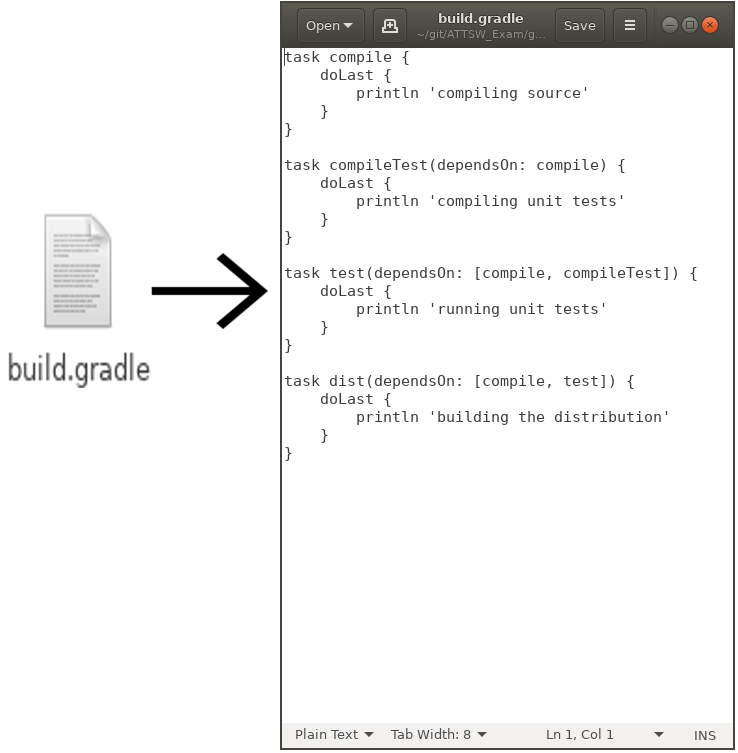
\includegraphics[scale=0.46]{gradleexamplefirst.png}
\end{figure} 
abbiamo creato un albero di dipendenze tra tasks di questo tipo:
\label{taskdip}
\begin{figure}[H]

\includegraphics[scale=0.70]{taskdipendence.png}
\end{figure}
è possibile fare diverse build con questa configurazione:
\begin{itemize}
    \item \begin{verbatim} $ gradle compile \end{verbatim}
    \item \begin{verbatim} $ gradle compileTest \end{verbatim}
    \item \begin{verbatim} $ gradle test \end{verbatim}
    \item \begin{verbatim} $ gradle dist \end{verbatim}
    \item una combinazione qualunque di 2 o più task.
\end{itemize}
Possiamo notare che anche se eseguiamo la build: 
\begin{verbatim}
    $ gradle compile test \end{verbatim}
il task \textbf{compile} verrà eseguito solo una volta:
\begin{verbatim}
> Task :compile 
compiling source

> Task :compileTest 
compiling unit tests

> Task :test 
running unit tests


BUILD SUCCESSFUL in 0s
3 actionable tasks: 3 executed \end{verbatim}

\subsubsection{Escludere task da una build}
È possibile escludere un task di una build, aggiungendo come argomento il task da escludere preceduto da -x:
\begin{verbatim}
    $ gradle <task_da_eseguire> -x <task_da_escludere> \end{verbatim}
questo viene usato al fine di eliminare un task inutile per lo scopo della build che abbiamo intenzione di eseguire. Riprendendo l'esempio del paragrafo precedente se andiamo ad eseguire la build:
\begin{verbatim}
    $ gradle dist \end{verbatim}
vediamo che vengono eseguiti tutti i tasks, compresi i tasks \textbf{test} e \textbf{compileTest}, supponendo di voler fare solo la build del sorgente possiamo scrivere:
\begin{verbatim}
    $ gradle dist -x test
\end{verbatim}
l'output risultante sarà:
\begin{verbatim}
> Task :compile 
compiling source

> Task :dist 
building the distribution


BUILD SUCCESSFUL in 0s
2 actionable tasks: 2 executed \end{verbatim}
Il task \textbf{compileTest} non viene eseguito perchè dipendenza di \textbf{test}, ma non di \textbf{dist} (vedi pag. \pageref{taskdip}), escludendo il primo quindi non è necessario eseguire il task \textbf{compileTest}. Nel file di configurazione della build è possibile inserire anche un descrizione inserendo in testa al file build.gradle la seguente riga:
\begin{verbatim}
    description = 'Descrizione' \end{verbatim}
Questo è importante per progetti multi-builds consentendo di avere una descrizione di ogni singola build.

\subsubsection{Abbreviazione del nome del task} è possibile abbreviare il nome del task da eseguire stando però attenti ad identificare unicamente il task che vogliamo eseguire, per esempio se volessi eseguire il task \textbf{compileTest} potrei farlo semplicemente con il comando:
\begin{verbatim}
    $ gradle comTes \end{verbatim}
considerando i task creati precedentemente notiamo che il task è univocamente identificato.

\subsubsection{Selezionare la build da eseguire} consideriamo che esista in una subdirectory chiamata subdir una build chiamata subbild.gradle, partendo dalla directory root è possibile eseguire questa build eseguendo il comando:
\begin{verbatim}
    $ gradle -b subdir/subbuild.gradle <task_da_eseguire> \end{verbatim}
è possibile anche indicare direttamente la project directory da usare, nel nostro caso indicheremo subdir:
\begin{verbatim}
    $ gradle -p subdir  \end{verbatim}

\subsubsection{Forzare l'esecuzione di un task} a causa della Gradle cache è possibile che un task o più di uno non vengano eseguiti perchè marcati come UP-TO-DATE (anche se dalla versione Gradle 4.0 non viene più mostrato in output), in questo caso è possibile forzarne l'esecuzione con:
\begin{verbatim}
    $ gradle --rerun-tasks <tasks_da_eseguire> \end{verbatim}

\subsubsection{Ottenere informazioni generali} come già detto precedentemente nel caso di progetti multi-builds è necessario avere una descrizione di ogni file di configurazione della build, per ottenere le informazioni sul progetto corrispondente alla build è possibile eseguire il task \texttt{projects}:
\begin{verbatim}
    $ gradle projects \end{verbatim}

\subsubsection{Ottenere informazioni sui tasks} è possibile ricavare una lista dei tasks default eseguendo la build del task \texttt{tasks}:
\begin{verbatim}
    $ gradle tasks \end{verbatim}
possiamo notare che l'output non mostra tutti i task, ma solo quelli predefiniti:
\begin{verbatim}
> Task :tasks 

------------------------------------------------------------
All tasks runnable from root project - Descrizione
------------------------------------------------------------

Build Setup tasks
-----------------
init - Initializes a new Gradle build.
wrapper - Generates Gradle wrapper files.

Help tasks
----------
buildEnvironment - Displays all buildscript dependencies declared in root project 'first'.
components - Displays the components produced by root project 'first'. [incubating]
dependencies - Displays all dependencies declared in root project 'first'.
dependencyInsight - Displays the insight into a specific dependency in root project 'first'.
dependentComponents - Displays the dependent components of components in root project 'first'. [incubating]
help - Displays a help message.
model - Displays the configuration model of root project 'first'. [incubating]
projects - Displays the sub-projects of root project 'first'.
properties - Displays the properties of root project 'first'.
tasks - Displays the tasks runnable from root project 'first'.

To see all tasks and more detail, run gradle tasks --all

To see more detail about a task, run gradle help --task <task>


BUILD SUCCESSFUL in 0s
1 actionable task: 1 executed \end{verbatim}
come dice l'output, per visualizzare la lista di tutti i tasks è necessario eseguire la build del task \texttt{tasks} con argomento --all:
\begin{verbatim}
    $ gradle tasks --all \end{verbatim}
    il risultato sarà molto più specifico rispetto al precedente. Possiamo notare che a differenza degli altri tasks quelli che abbiamo creato noi sono sprovvisti di una descrizione, per aggiungerla basterà inserire un campo \texttt{description} all'interno della definizione del task:
    \begin{verbatim}
task dist(dependsOn: [compile, test]) {
    description = 'Build distribution'
    doLast {
        println 'building the distribution'
    }
} \end{verbatim}
rieseguendo il comando sopra otterremo una descrizione anche per il \texttt{dist}. Per ottenere informazioni più specifiche è possibile usare la build del task help seguito da --task e il nome del task:
\begin{verbatim}
    $ gradle help --task <task> \end{verbatim}
quello che vedremo sarà un riepilogo generale del task.

\subsection{Secondo tutorial: Gradle Wrapper}
Molto spesso prima di poter usufruire di uno strumento di sviluppo è necessaria una installazione. Gradle mette a disposizione uno script che permette di usare tutte le sue funzionalità evitando di installare Gradle su tutte le macchine di sviluppo, questo strumetno viene chiamato Gradle Wrapper. Se in un progetto è stato settato il Wrapper è possibile eseguire le builds direttamente dalla root del progetto con il comando:
\begin{verbatim}
    $ ./gradlew <task> \end{verbatim}
Se più persone lavorano a un progetto può capitare che ci siano differenze tra le versioni di uno strumento, nel caso del wrapper non è possibile sbagliare perchè la sua versione è insita durante la sua creazione o durante il suo upgrade (o downgrade). Quindi è sempre consigliato l'uso del wrapper e lasciare tutte le sue informazioni anche nella cartella principale del VCS usato.

\subsubsection{Aggiungere il Wrapper ad un progetto}
Per poter usufruire del wrapper è necessario eseguire il comando:
\begin{verbatim}
    $ gradle wrapper \end{verbatim}
è possibile trovare le versioni del Wrapper nella directory locale in cui è stato installato Gradle solitamente \textit{\$HOME/.gradle/wrapper/dists}. Il comando precedente creerà 4 files:
\begin{itemize}
    \item \textbf{gradlew}: script del wrapper per sistemi Unix
    \item \textbf{gradlew.bat}: file batch per sistemi Windows
    \item \textbf{gradle/wrapper/gradle-wrapper.properties}: proprietà del wrapper
    \item \textbf{gradle/wrapper/gradle-wrapper.jar}: file jar del wrapper
\end{itemize}
per usare una versione Gradle specifica è possibile usare 3 metodi:
\begin{enumerate}
    \item eseguire il solito comando con l'aggiunta dell'argomento --gradle-version:
\begin{verbatim}
    $ gradle wrapper --gradle-version <numero_versione> \end{verbatim}
oppure se già inserito il wrapper:
\begin{verbatim}
    $ ./gradlew wrapper --gradle-version <numero_versione> \end{verbatim}
per esempio se volessimo passare dalla versione 4.4.1 alla versione 2.0 basterà eseguire il comando:
\begin{verbatim}
    $ ./gradlew wrapper --gradle-version 2.0 \end{verbatim}
per aggiornare la versione gradle usata dal wrapper basterà eseguire:
\begin{verbatim}
    $ ./gradlew wrapper \end{verbatim}
    \item modificare direttamente il file gradle-wrapper.properties in cui nell'ultima riga ci sarà la versione usata dal Wrapper:
\begin{verbatim}
    distributionUrl=https\://services.gradle.org/distributions/gradle-4.4.1-bin.zip \end{verbatim}
    per passare alla versione 2.0 possiamo modificare questa riga con:
\begin{verbatim}
    distributionUrl=https\://services.gradle.org/distributions/gradle-2.0-bin.zip \end{verbatim}
    \item infine possiamo modificare la definizione del task \texttt{wrapper} della build di gradle, per farlo è necessario creare (se non è già stato fatto) il file build.gradle e aggiungere:
\begin{verbatim}
    task wrapper(type: Wrapper) {
        gradleVersion = '2.0'
    } \end{verbatim}
    ed eseguire nuovamente il task \texttt{wrapper}:
\begin{verbatim}
    $ ./gradlew wrapper \end{verbatim}
\end{enumerate}
in ogni caso possiamo visualizzare la versione usata dal wrapper con il comando:
\begin{verbatim}
    $ ./gradlew --version \end{verbatim}

\end{flushleft}
\end{document}
